\documentclass[capstone_report.tex]{subfiles}
\begin{document}
\chapter*{Executive Summary}                                
\addcontentsline{toc}{chapter}{Executive Summary} 
The recent increase in the availability of small, battery powered, unmanned aircraft has opened up an interesting vista for robotics and artificial intelligence. Unlike their ground-based cousins, UAVs can enter and monitor indoor environments even in the presence of uneven or broken ground. This is not currently practical for wheeled robots. \\

Applications for UAVs which can enter, navigate and observe indoor environments are obvious and numerous, ranging from mapping out the geology of an underground mine, to assisting emergency services personnel in locating people inside a building. In the world of fiction, automated UAVs exploring an environment and reporting back to their masters with a touch of a button already feature heavily, and are typically used where direct exploration by humans is not possible.\\

Of course, in the real world it is never so simple. Limitations such as battery life, sensor accuracy, clutch exploration decisions, converting observations into reliable mapping information, pathfinding, cooperation, transient obstacles and many other edge cases mean that so far, no singe product can reliably navigate indoor environments without a pilot.\\

Our project is aimed to design a bare-bones prototype which tackles some of these challenges. We show the design of an Unmanned Recon and Safety Aircraft (U.R.S.A.) which can navigate in a number of basic indoor environments without human intervention. While we do not claim to have overcome every limitation outlined above, we offer this as an important first step towards fully autonomous indoor aerial vehicles. \\

This project was developed under the guidance of the Melbourne Metro Fire Brigade (MFB). MFB has been an early adopter of UAVs for emergency situations, and have a large fleet of UAVs and accredited pilots in operation. MFB have sponsored this project in an attempt to further advance the state of the art regarding UAVs applied in emergency situations.\\

The final product delivered consists of a UAV which can navigate in both a simulated environment, and in a real world scenario. The primary mechanism of navigation is 2D laser scan data. Range measurements are taken in a \SI{240}{\degree} arc, and these are converted to a joint estimate of URSA's position and surrounding obstacles. A sampling approach is then used for pathfinding. Figure \ref{fig:sim} shows URSA in simulation, and Figure \ref{fig:real} shows the real-world prototype. \\


    \begin{figure}  [H]
	\centering
        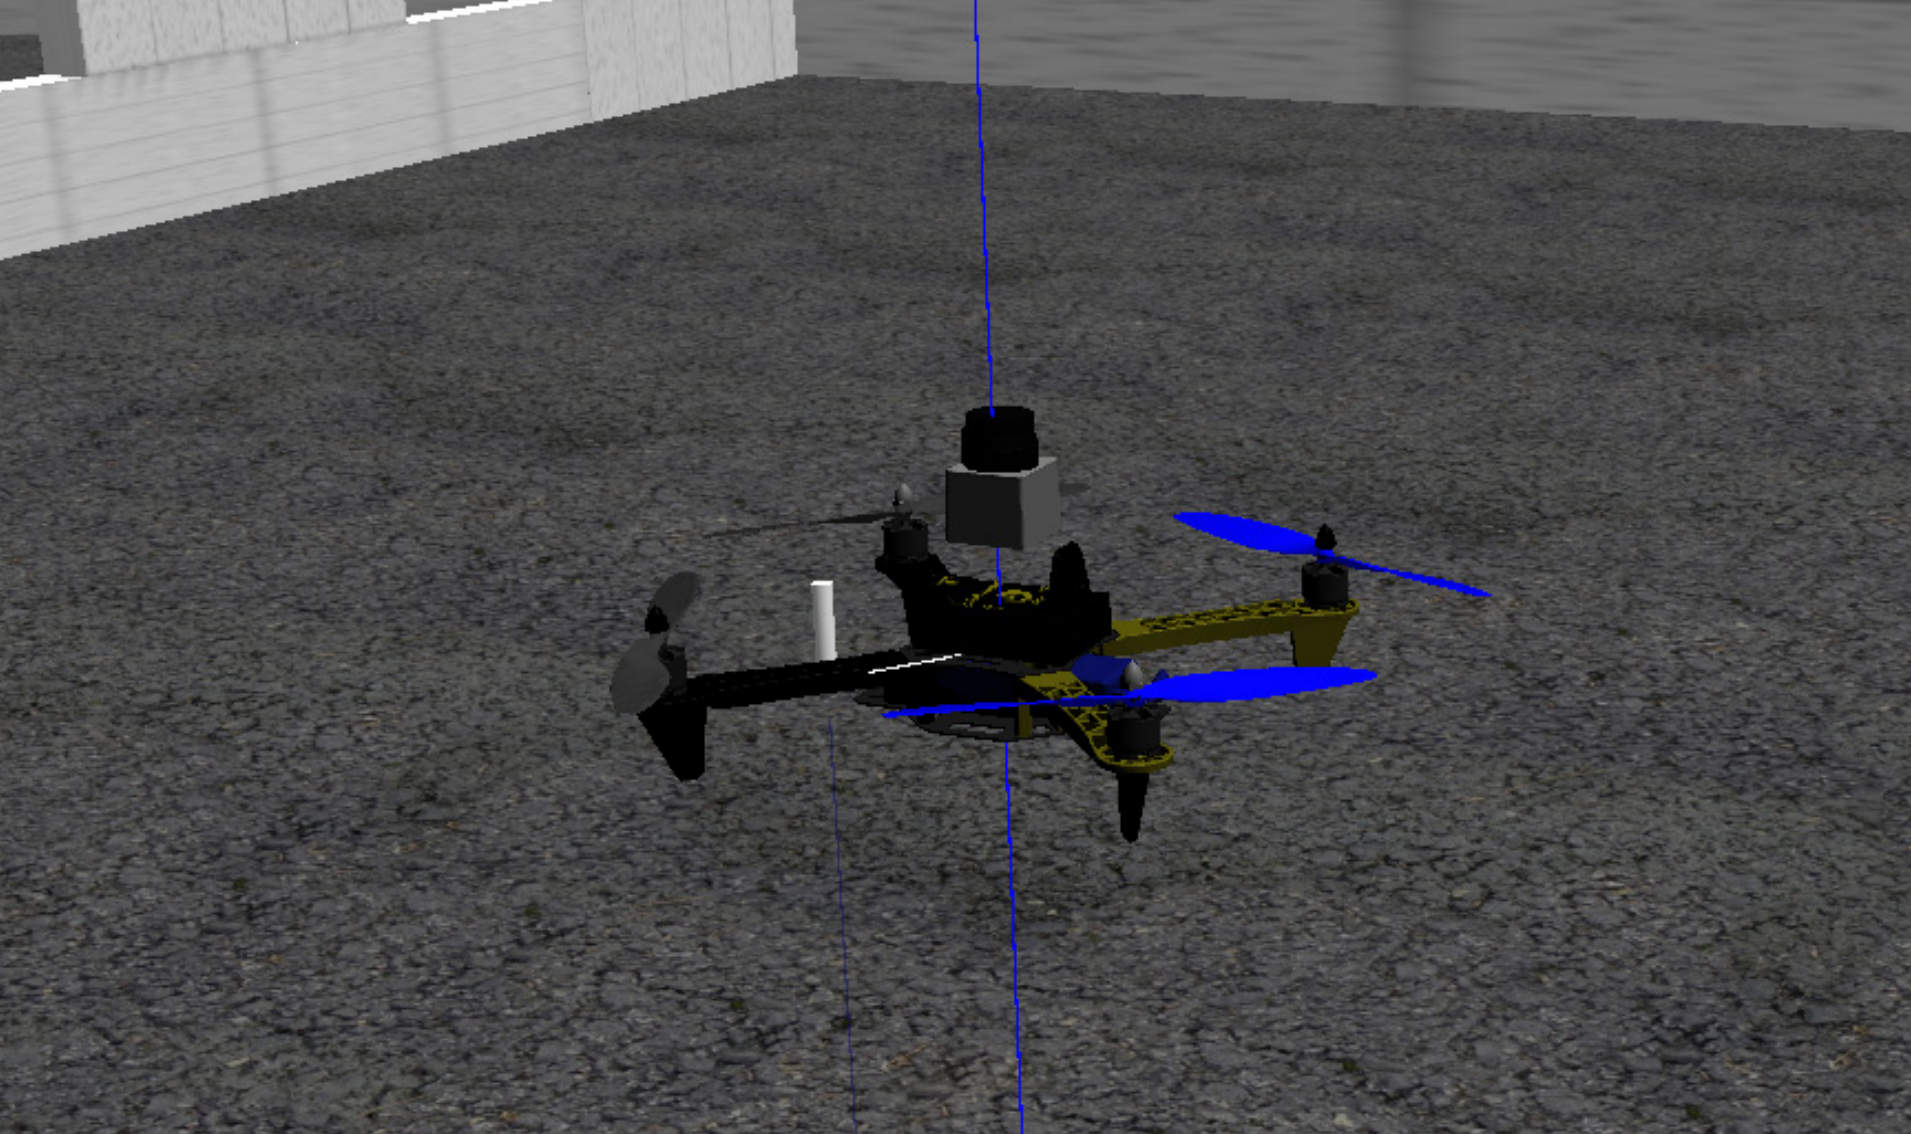
\includegraphics[width=0.6\linewidth]{imgs/simulation.png}
        \captionof{figure}{URSA in simulation}
        \label{fig:sim}
    \end{figure}


    \begin{figure}  [H]
	\centering
        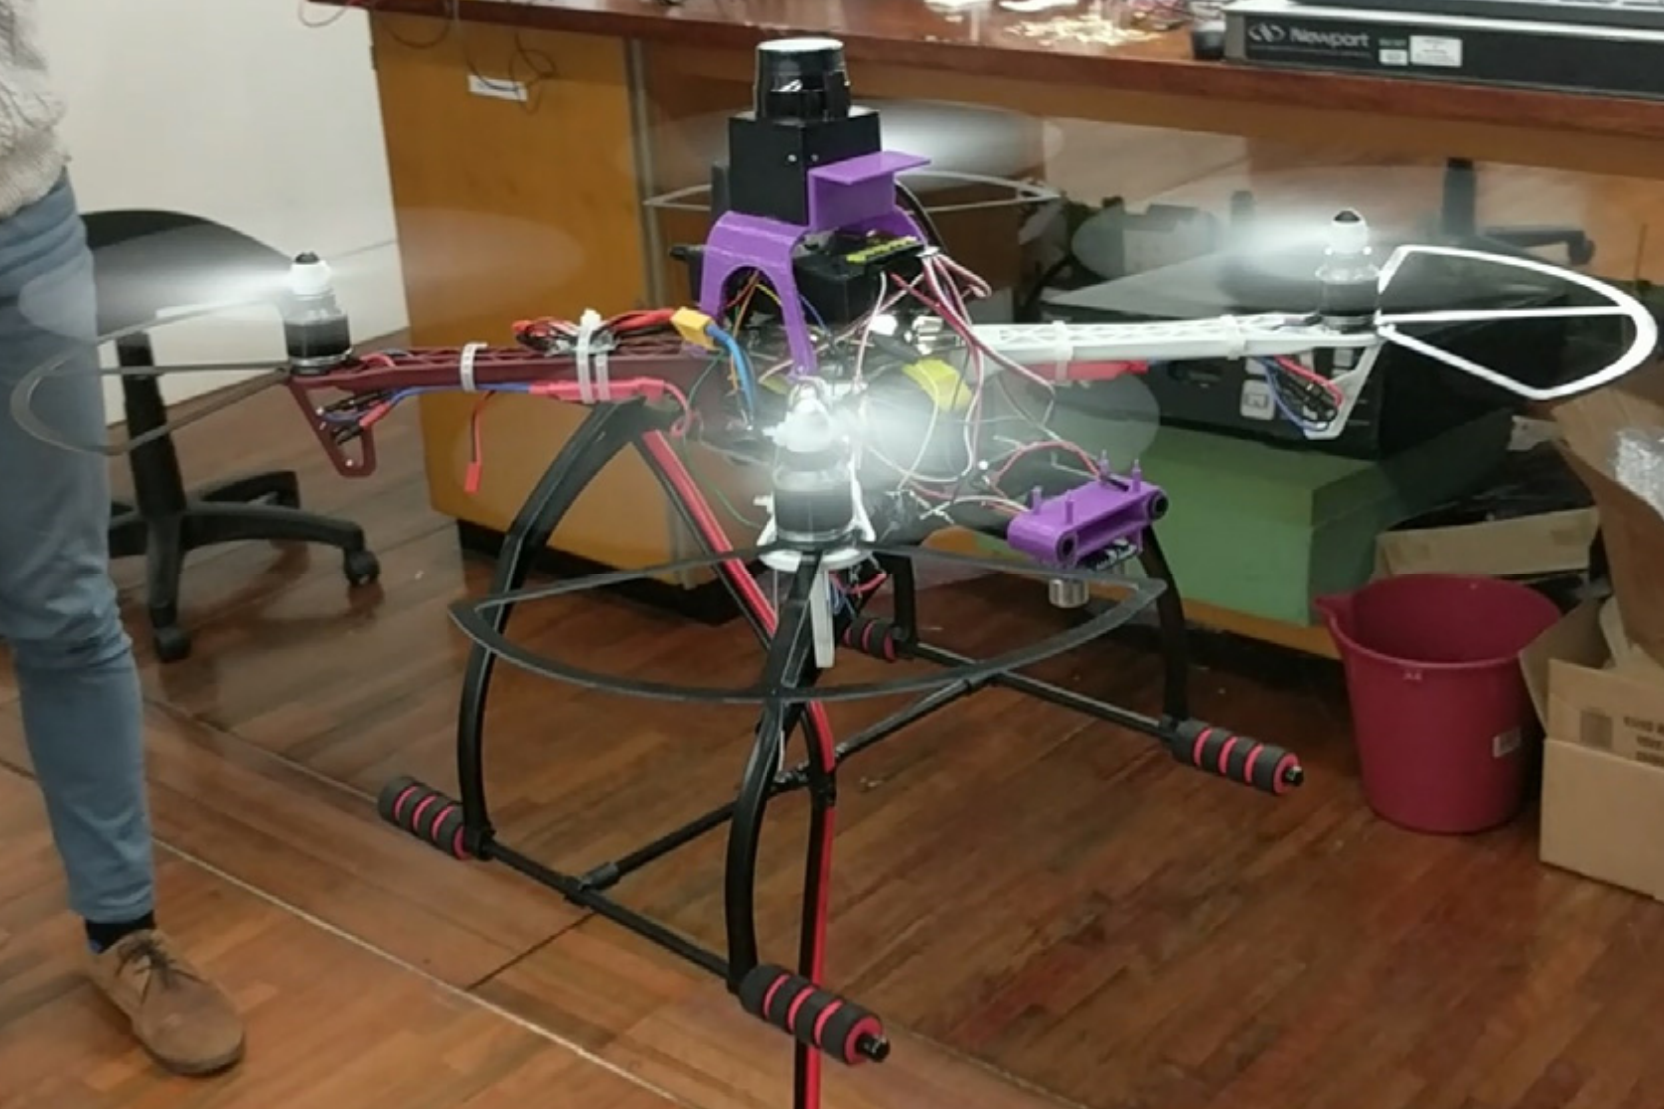
\includegraphics[width=0.6\linewidth]{imgs/real.png}
        \captionof{figure}{URSA real world prototype}
        \label{fig:real}
    \end{figure}

The results of URSA are extremely promising for indoor UAV navigation in future. While large complications and barriers still exist to practical, real-world deployment, it is likely that these can be overcome through refining the URSA product and addressing edge cases.\\

This report is structured into four main chapters. The first chapter focuses on the preliminary work undertaken to gather requirements and ensure proper project management was in place. The second chapter focuses on the technical design of the URSA system. The third chapter relates to the effort expended in developing this system. The fourth and final chapter detail our test results and areas for further development. Appendices are provided, including datasheets for all relevant components. Due to the volume of code developed, code has not been provided but is available on GitHub at \url{http://www.github.com/ursa-drone}.

As the reader of this report, we hope you are excited by the results shown and the future applications URSA may have to improved emergency services aircraft.

\end{document}